\chapter{Introduction}
\label{sec:introduction}

This section contains some things you will often use in a thesis.

In the following a paper found in literature.bib is cited \cite{empe:2002th}.

Use TIKZ to draw a graph as shown in figure \ref{fig:splits}.

\begin{figure}
\centering
\begin{subfigure}[b]{0.5\textwidth}
	\centering
	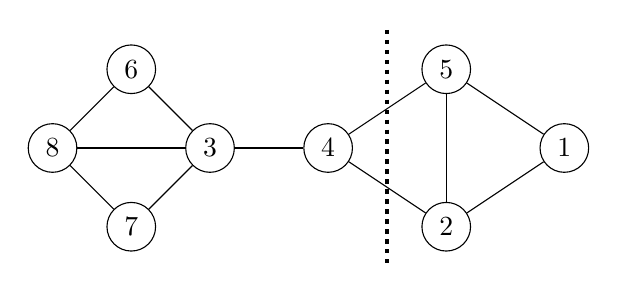
\begin{tikzpicture}[scale=.5,auto=left,every node/.style={draw,circle}]
		\node (n8) at (-2,8) {8};
		\node (n7) at (0,6)  {7};
		\node (n6) at (0,10) {6};
		\node (n4) at (5,8)  {4};
		\node (n5) at (8,10) {5};
		\node (n1) at (11,8) {1};
		\node (n2) at (8,6)  {2};
 		\node (n3) at (2,8)  {3};

		\foreach \from/\to in {n6/n3,n4/n5,n5/n1,n1/n2,n2/n5,n2/n4,n3/n4,n8/n6,n8/n7,n8/n3,n7/n3}
	    	\draw (\from) -- (\to);
		\draw [dotted, ultra thick] (6.5,11) -- (6.5,5);
	\end{tikzpicture}
	\caption{Non-optimal Split}
\end{subfigure}
\begin{subfigure}[b]{0.5\textwidth}
	\centering
	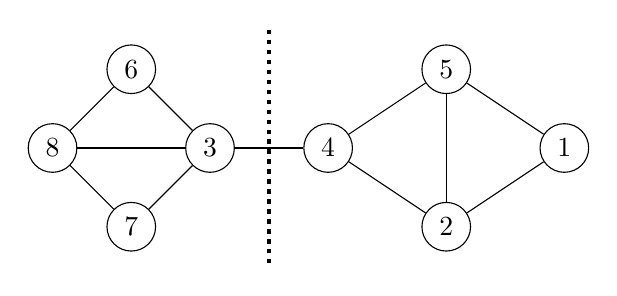
\begin{tikzpicture}[scale=.5,auto=left,every node/.style={draw,circle}]
		\node (n8) at (-2,8) {8};
		\node (n7) at (0,6)  {7};
		\node (n6) at (0,10) {6};
		\node (n4) at (5,8)  {4};
		\node (n5) at (8,10) {5};
		\node (n1) at (11,8) {1};
		\node (n2) at (8,6)  {2};
 		\node (n3) at (2,8)  {3};

		\foreach \from/\to in {n6/n3,n4/n5,n5/n1,n1/n2,n2/n5,n2/n4,n3/n4,n8/n6,n8/n7,n8/n3,n7/n3}
	    	\draw (\from) -- (\to);
		\draw [dotted, ultra thick] (3.5,11) -- (3.5,5);
	\end{tikzpicture}
	\caption{Optimal Split}
\end{subfigure}
\caption{Splits in Structural Graph Partitioning}
\label{fig:splits}
\end{figure}

\begin{itemize}
	\item This is an item
	\item And this is another one
\end{itemize}

Include a PDF as a picture. How about this CAB (Compute Aggregate Broadcast) diagram shown in figure \ref{img:arch}.

\cpic{imgs/dgms/bsp-basic.pdf}{Compute Aggregate Broadcast computing paradigm}{img:arch} 

How about another picture with a state machine \ref{fig:globalpregelstate}?

\begin{figure}
\centering
	\begin{tikzpicture}[->,>=stealth,scale=.4,auto=left,every node/.style={}]
		\tikzset{state/.style={draw,ellipse}}
		\tikzset{start/.style={}}
		\tikzset{textlabel/.style={}}

		\node [start] (start) at (0, 12) {started} ;
		\node [state] (init) at (0, 9)  {init} ;
		\node [state] (processing) at (0, 6)  {processing} ;
		\node [state] (messaging) at (0, 3) {messaging} ;
		\node [state] (global) at (10, 4.5) {global} ;
		\node [start] (end) at (0, 0) {terminated} ;

		\path (start) edge (init);
		\path (init) edge (processing);
		\path (processing) edge (messaging);
		\path (messaging) edge (end);
		\path (messaging) edge [bend right] (global);
		\path (global) edge [bend right] (processing);

		\node [textlabel] (continue) at (7, 1) {\emph{activeVertices > 0}};
		\node [textlabel] (halt) at (-5, 1) {\emph{activeVertices = 0}};
	\end{tikzpicture}
\caption{Global State Machine}
\label{fig:globalpregelstate}
\end{figure}

Or include some Java code.

\lstinputlisting[caption={HelloWorld}, language=Java, firstline=3, lastline=9, label=lst:pagerank]{code/HelloWorld.java}
